\begin{figure}[t]
\centering
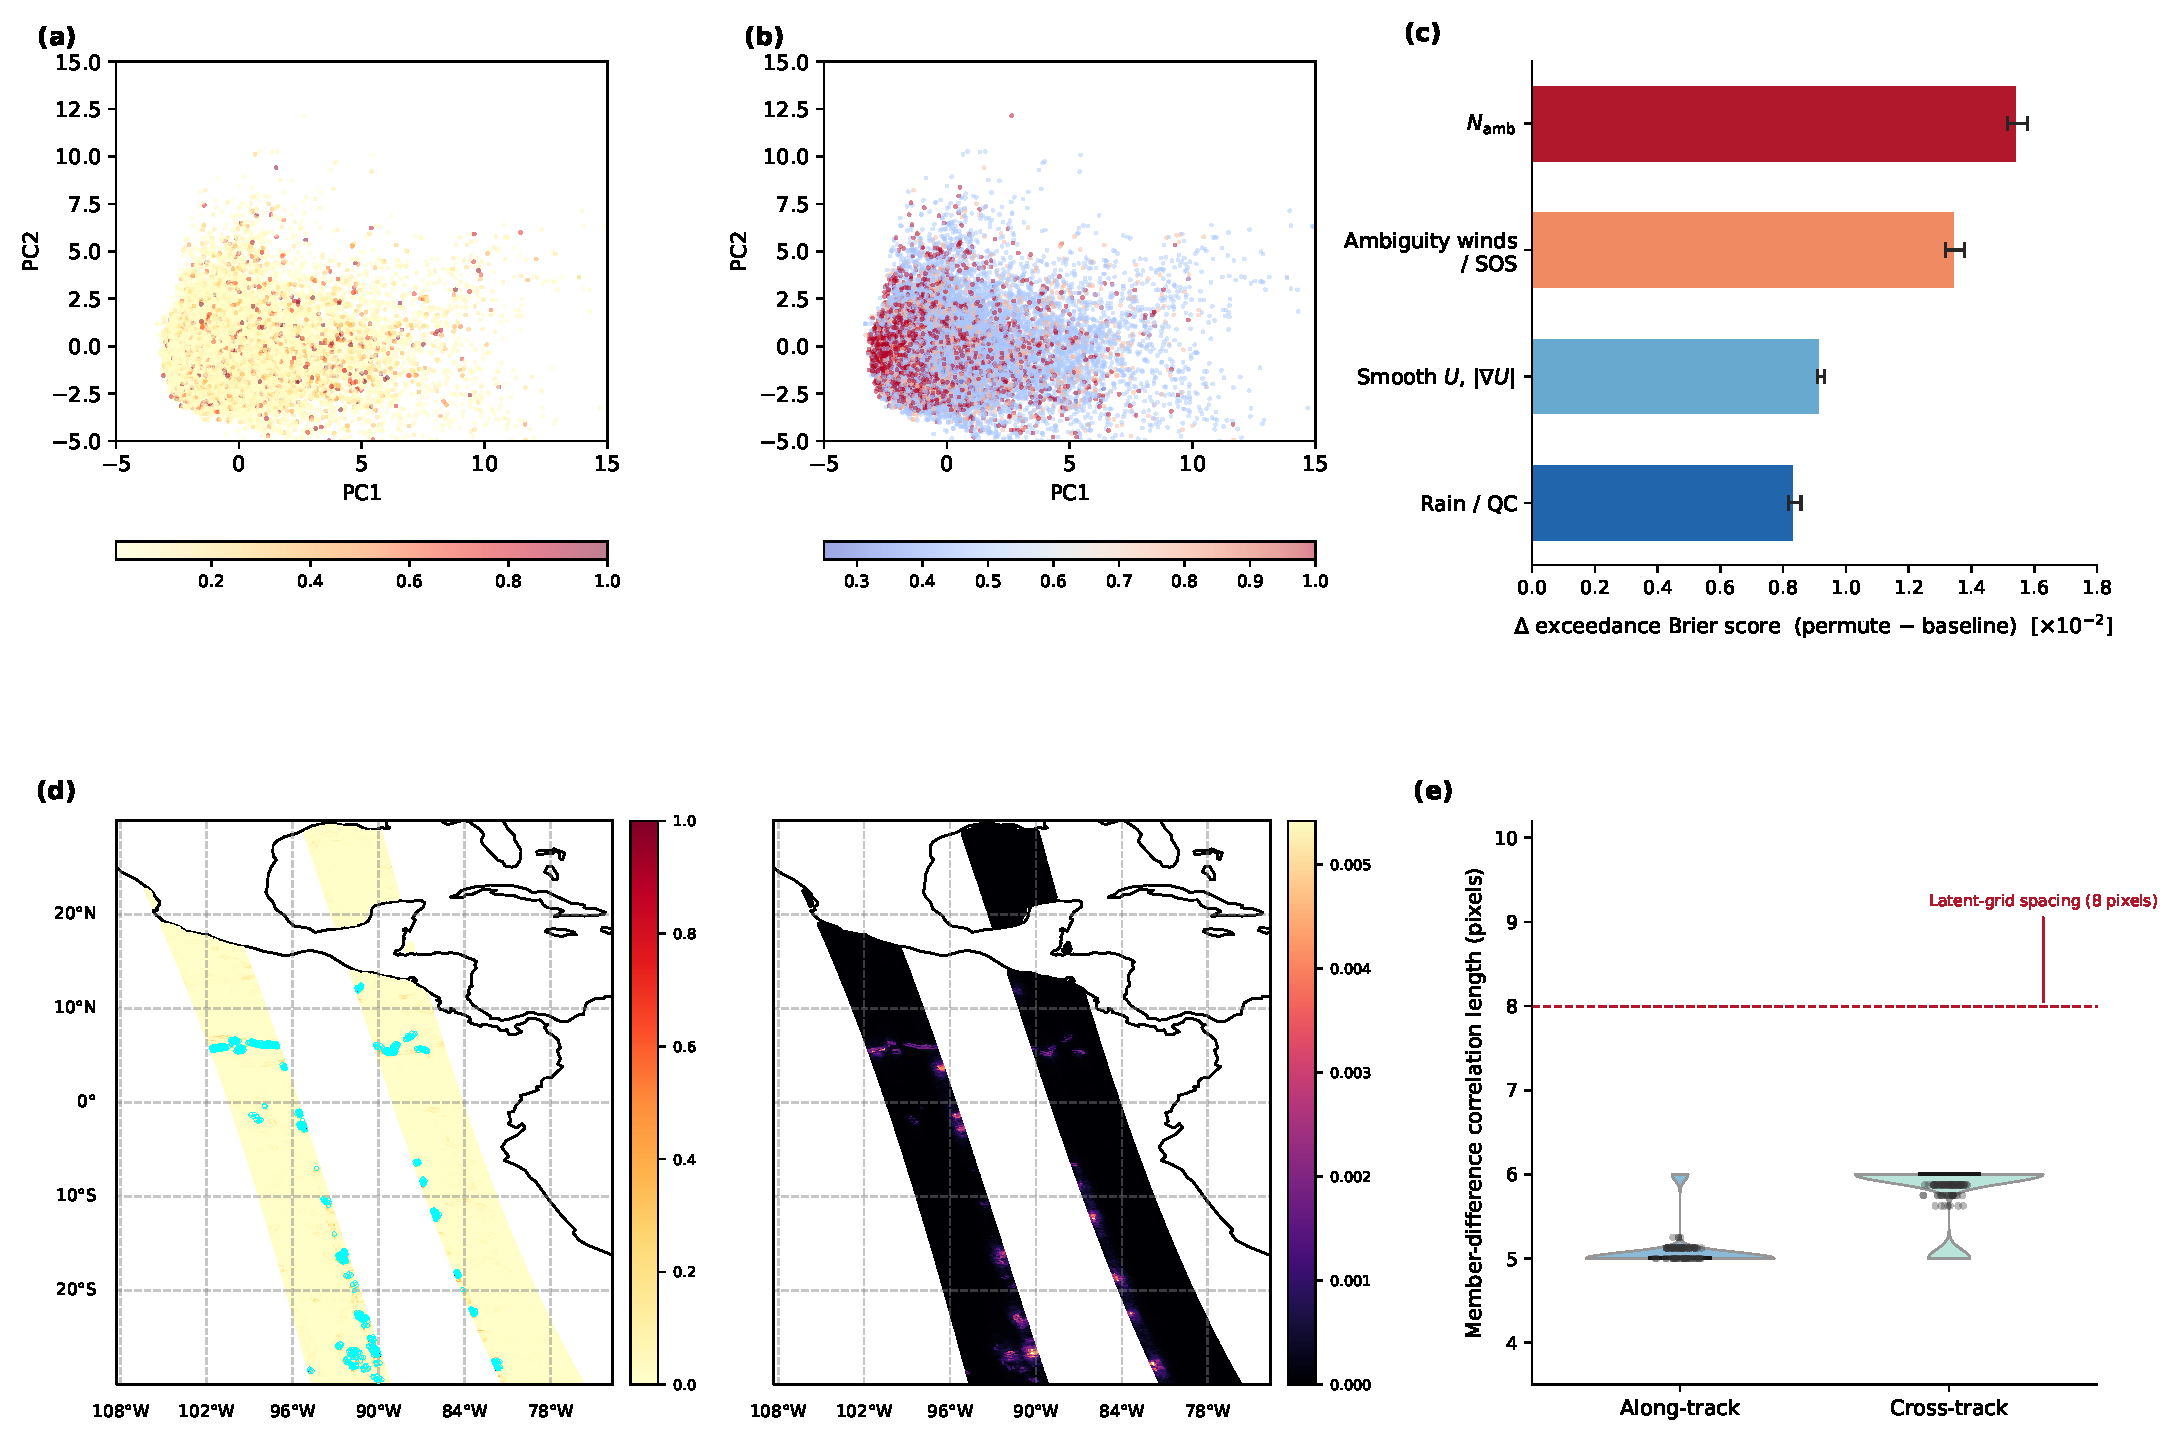
\includegraphics[width=\textwidth]{13_explainability_main.pdf}
\caption{Learned representation, attribution, and ensemble coherence for the
CRPS ensemble U-Net.
(a)~Bottleneck PCA colored by soft exceedance probability $P(S>\tau^*)$.
(b)~Same embedding colored by ambiguity count $N_{\mathrm{amb}}$.
(c)~Predictor-group along-track permutation importance for the exceedance
Brier score at $\tau^*=1.2\times10^{-4}$ (mean $\Delta$score $\pm$ SD over
latent seeds $\times$ permutation draws). Ambiguity predictors exceed smooth
context; uncertainties are small relative to group differences.
(d)~Integrated gradients on a representative ASCAT swath (lon/lat scatter):
$P(S>\tau^*)$ and $|\mathrm{IG}|$ summed over input channels (cyan: high-$P$ ROI).
(e)~Member-difference correlation length of ensemble deviations from the
member mean: along-track and cross-track $L$ concentrate near 5--6~pixels.
The dashed line marks the latent-grid spacing (8~pixels) of the stochastic
noise input; member diversity therefore sits at the noise-grid scale rather
than at long front-scale modes.
Corresponding afCRPS permutation numbers and latent $z$-traversal cases appear
in the Supporting Information.}
\label{fig:explainability}
\end{figure}
